\chapter{Einleitung}
%\vspace{-1.2cm}\todo{eventuel einfach löschen}
%Im folgenden Kapitel wird die Grundlage für die vorliegende Bachelorarbeit geschaffen. Hierbei werden die Motivation und das Ziel der Arbeit erläutert, um einen klaren Überblick über den Themenkontext zu bieten. Des Weiteren werden die Anforderungen an das System gestellt.

\section{Pepperl + Fuchs / HMI}\label{sec:PFHMI}
Die Firma \acl{p+f} wurde 1945 von Walter Pepperl und Ludwig Fuchs gegründet. Anfangs war sie eine Radioreparaturwerkstadt, welche sich erst nach der Entwicklung eines eigenen Näherungsschalters sowie eines eigensicheren Transistorverstärkers auf das Gebiet der Elektronik ausweitete. Inzwischen entwickelt, produziert und vertreibt \ac{p+f} Baugruppen und Sensoren für den Automatisierungsmarkt. \cite{PFGeschichte}\\
\vspace{-1cm}
\begin{flushleft}
    \begin{figure}[h!]
        \centering
        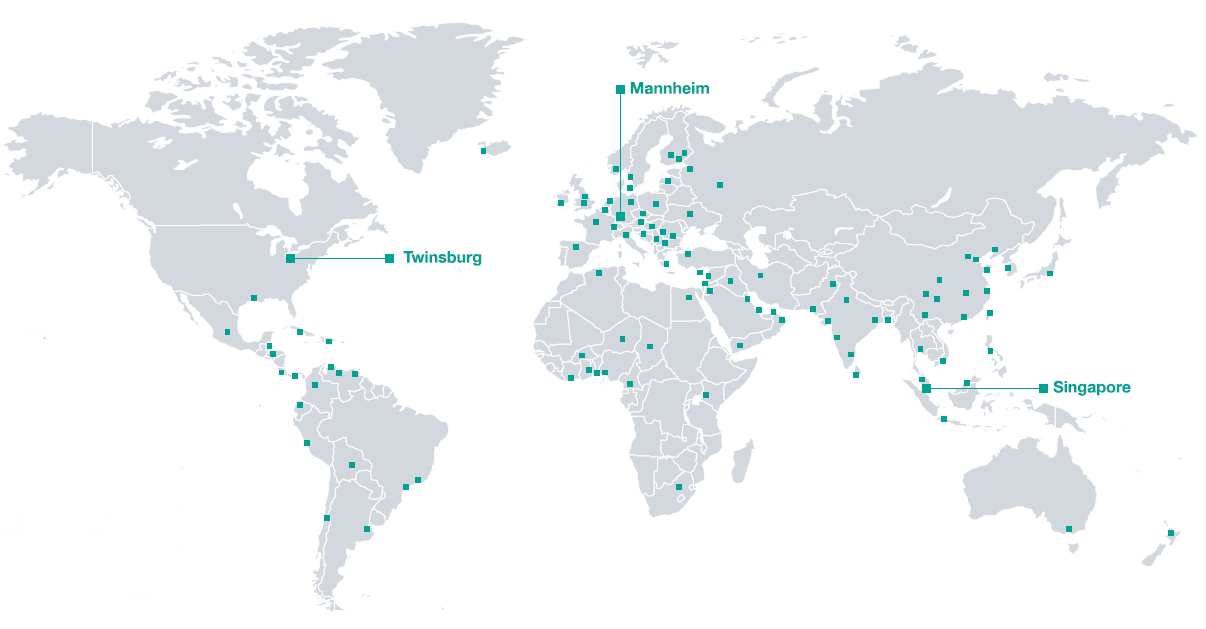
\includegraphics[width=1\linewidth]{P+F_Standorte.png}
        \caption{Standorte der Pepperl+Fuchs SE}
        \label{fig:StandortePF}
    \end{figure}
\end{flushleft}
Im Bereich der Prozessautomation ist \ac*{p+f} führender Hersteller industrieller Sicherheitsausstattungen. Das Produktportfolio umfasst eine Reihe industrieller Computersysteme, welche zur Überwachung und Steuerung von Prozessen in explosionsgefährdeten Bereichen genutzt werden. Die \ac{hmi} Abteilung beschäftigt sich mit der Entwicklung dieser Systeme, welche eine Schnittstelle zwischen Mensch und Maschine bilden. Da es eine Vielzahl an Anwendungen für \ac{hmi} Systeme in explosionsgefährdeten Bereichen gibt, wurde die Produktfamilie \textit{VisuNet} speziell für den Einsatz in diesen Zonen konzipiert. 
Solche Ex-Zonen sind überall da zu finden, wo explosionsgefährliche Stoffe gelagert oder gehandhabt werden. In diesen Zonen kann durch Gas oder Staub, eine explosionsfähige Atmosphäre entstehen. Zudem kommen auch umwelttechnische Einflüsse wie Sonne, Nässe, Hitze und Kälte, aber auch Einflüsse, welche beispielsweise durch die Reinigung mit aggressiven Chemikalien entstehen, hinzu. 
Um in solchen Computer feindlichen Umgebung dennoch ein Prozessleitsystem zu integrieren, setzte \ac{p+f} mit den \textit{VisuNet} Remote Monitoren auf die Thin-Client-Technologie. Hierbei verbindet sich der Ex-Geschützte Monitor aus der Explosionsgefährdeten Zone mit der Zentralen, meist leistungsstärkeren, Recheneinheit in der No-Ex-Zonen. Eingaben über Tastatur und Maus werden anschließend über den Monitor an die Zentrale Recheneinheit weitergeleitet, welche anschließend die neuen Ausgaben an den Monitor zurückschickt. \cite{HMIYannick}\todo{Bild der HMI Geräte einfügen}

\section{Intention und Ziel der Arbeit}\label{sec:IZA}
Durch die Ex-Schutzzertifizierung der \textit{VisuNet} Plattformen, sind vorgeschriebene Betriebstemperaturgrenzen der Systeme einzuhalten. Integrierte Schutzschaltungen und weitere Sicherheitsmechanismen hindern die Geräten daran, diese Grenzwerte zu überschreiten. Umwelteinflüsse, wie beispielsweise die Sonneneinstrahlung oder Vibrationen, der industriellen Umgebungen in welchen die Geräte operieren, können negative Auswirkung auf die Systeme haben. Zudem können solche Umwelteinflüsse Gerät in Systemzustände bringen, welche den Zertifizierungsrichtlinien widersprechen. Durch eine falsche Einschätzung der Umweltfaktoren werden unzulässige bzw. schädliche Betriebe vom Endkunden meist nicht wahrgenommen.\\
Eine Möglichkeit dem zu begegnen, ist die auf der Hardware verbaute Sensorik zu nutzen, um den Zustand des Systems zu überwachen. Aus den Daten können anschließend Rückschlüsse auf Betriebszustände und das daraus resultierende Nutzungsverhalten gezogen werden. Dem Nutzer können somit wichtige Informationen zum Systemzustand vermittelt werden, sodass schädliche bzw. unzulässige Zustände entdeckt und vermieden werden können.\\
Primäres Ziel dieser Bachelorarbeit ist daher, die prototypische Entwicklung einer Hardware-Health-Monitoring Lösung für die \ac{p+f} \ac{hmi} Plattformen \textit{VisuNet GXP} und \textit{FLX}. Hierbei soll eine Architektur und Konzepterweiterung für den Aufbau einer verteilten Health-Monitoring Lösung, welche möglichst plattformunabhängig ausgeführt werden kann, erstellt werden. Dazu gilt es Sensoren und Messwerte, die bei der„Health"-Status Definition berücksichtigt werden sollen, auszuwählen und auszulesen. Des Weiteren soll ein Modell definiert werden, welches die Sensor-Messwerte in einen plattformspezifischen Health-Status übersetzt, um dem Benutzer den aktuellen Zustand mitzuteilen. Als prototypische Umsetzung, soll ein Health Agent entwickelt werden, welcher Geräte-Daten (z.B. aktuelle Temperatur) der \ac{hmi}-Systeme ausliest, abspeichert, in der VisuNet RM Shell 6 dem Benutzer visualisiert und per Netzwerkprotokoll (z.B. MQTT oder SNMP) einem zentralen Server bereitstellen kann.    

\section{Anforderungen}\label{sec:Anforderungen}\todo{Anforderungen etwas mehr ausformulieren}
Durch das in Abschnitt \ref{sec:IZA} erläuterte Ziel dieser Arbeit ergeben sich die unten aufgelisteten Anforderungen.
\begin{enumerate}
    \item \textbf{Datenerfassung}
    \begin{enumerate}
        \item \textbf{Auslesen der Systemsensorik}\\
        Das System benötigt eine zentrale Schnittstelle, welche das Auslesen der Sensoren der \textit{VisuNet} Plattformen ermöglicht. Die \textit{VisuNet} Plattformen unterscheiden sich in der ausgestatteten Elektronik so weit, dass verschiedene Ansätze zum Auswerten dieser benötigt werden, um eine plattformunabhängige Benutzung der Anwendung zu ermöglichen. 
        \item \textbf{Speichern der ausgelesenen Messwerte}\\
        Zur Verwaltung der gesammelten Daten benötigt das System eine zentrale Datenbank. Diese muss über eine übersichtliche und effiziente Struktur verfügen, welche das Verarbeiten der gesammelten Daten im Nachgang ermöglicht. Des Weiteren muss die Struktur der Datenbank in der Lage sein, Sensorwerte verschiedener Geräte speichern zu können.
    \end{enumerate}
    
    \item \textbf{Datenverarbeitung}
    \begin{enumerate}
        \item \textbf{Ermittlung eines Health Status}\\
        Für die jeweiligen \textit{VisuNet} Plattformen soll ein System Health Status ermittelt werden. Dieser soll Aufschluss über den Betrieb des Systems geben und Nutzer über schädliche und unzulässige Betriebe informieren.  
        \item \textbf{Ermittlung einer Health Status Historie}\\
        Über die gesammelten Health Status Daten soll zudem eine Historie erstellt werden. Diese soll Aufschluss über das generelle Nutzungsverhalten des Systems geben. 
        \item \textbf{Ermittlung einer System Reliability}\\
        Zudem soll eine Aussage über den Zustand der im System verbauten Elektronik, mittels Reliability, getroffen werden. 
    \end{enumerate}

    \item \textbf{Datendistribution}
    \begin{enumerate}
        \item \textbf{Visualisierung der Systemdaten}\\
        Die gesammelten Daten des Systems sollen über ein Dashboard visualisiert werden. In diesem soll dem Kunden, eine Auswertung des Systemverhaltens präsentiert werden. Das Dashboard soll dabei von einem beliebigen Gerät aufrufbar sein.
        \item \textbf{Distribution der Daten zu einem externen Service}\\
        Die gesammelten Daten des Systems sollen über ein Netzwerkprotokoll (MQTT, SNMP, HTTP) an einen dritten Service übermittelt werden können.
    \end{enumerate}

   \end{enumerate}

